% !TEX root = ../ITGO.tex

In this problem, the objective is to minimize the cost of the gear ratio of the gear train \citep{PV}. An example is shown in Figure \ref{fig:GT}. The problem has four variables, representing the number of teeth for the four gears ($x_1 = A$, $x_2 = B$, $x_3 = D$, and $x_4 = F$), with $f(\bm{x}^*) = 2.700857E \! - \! 12$. The only constraint of the problem is that all variables must be integers. The full problem statement follows:

\vspace{-0.5cm}

\begin{align*}
\textbf{Minimize:} & \\
& f(\bm{x}) = \Big(\Big(\frac{1}{6.931}\Big) - \Big(\frac{x_2 x_3}{x_1 x_4} \Big)  \Big)^2 \\[0.5em]
\textbf{with bounds:} & \\
& 12 \leq x_i \leq 60, \quad i = 1, 2, 3, 4 \\
& x_i \in \mathbb{Z}, \quad i = 1, 2, 3, 4
\end{align*}

\vspace{0.5cm}


\begin{figure}[h]
    \begin{center}
    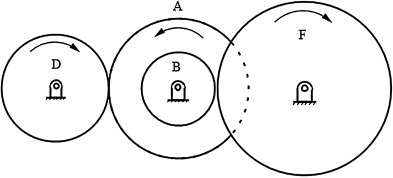
\includegraphics[scale=0.6]{Imgs/GT.jpg}
    \end{center}
    \captionsetup{justification=centering}
    \caption{Gear train design problem structure.}\label{fig:GT}
\end{figure}
